\documentclass[twocolumn]{el-author}

%\usepackage[...]{...}      This has been commented out as we are not using any additional packages here.  On the whole, they should be unnecessary.
\newcommand{\hH}{\hat{H}}
\newcommand{\D}{^\dagger}
\newcommand{\ua}{\uparrow}
\newcommand{\nc}{\newcommand}
\nc{\da}{\downarrow} \nc{\hc}{\hat{c}} \nc{\hS}{\hat{S}}
\nc{\bra}{\langle} \nc{\ket}{\rangle} \nc{\eq}{equation (\ref}
\nc{\h}{\hat} \nc{\hT}{\h{T}}\nc{\be}{\begin{eqnarray}}
\nc{\ee}{\end{eqnarray}}\nc{\rd}{\textrm{d}}\nc{\e}{eqnarray}\nc{\hR}{\hat{R}}\nc{\Tr}{\mathrm{Tr}}
\nc{\tS}{\tilde{S}}\nc{\tr}{\mathrm{tr}}\nc{\8}{\infty}\nc{\lgs}{\bra\ua,\phi|}\nc{\rgs}{|\ua,\phi\ket}
\nc{\hU}{\hat{U}}\nc{\lfs}{\bra\phi|}\nc{\rfs}{|\phi\ket}\nc{\hZ}{\hat{Z}}\nc{\hd}{\hat{d}}\nc{\mD}{\mathcal{D}}
\nc{\bd}{\bar{d}}\nc{\bc}{\bar{c}}\nc{\mc}{\mathcal}\nc{\ea}{eqnarray}\nc{\mG}{\mathcal{G}}\nc{\bce}{\begin{center}}
\nc{\ece}{\end{center}}
\date{12th December 2011}

\begin{document}

\title{Instructions and example template for \LaTeX{} submissions to \emph{Electronics Letters}}

\author{J. Smith and A. N. Other}

\abstract{This document describes how to use the el-author.cls file and how to format your \LaTeX submissions
correctly for \emph{Electronics Letters}. It also serves as a template, so that you can simply
copy the text from this example .tex file and replace it with your own.  We have tried to cover the basic
tools and commands you might need, but there may be some more unusual fields, etc, not described. Do not hesitate to contact
us if you encounter any problems.  The structure is as follows: we introduce the basic notations and preamble, and then provide some example text, followed by the references.  For simplicity we have left the source code out of this document and refer the reader to the sample.tex file itself, from which to copy and paste.}

\maketitle

\section{Introduction}

\verb"el-author.cls" is used in a similar fashion to the standard \verb"article.cls" file. However, the \verb"el-author.cls" file must be copied into the same directory as the .tex file you wish to compile for submission. Most of the preamble needed for including packages for mathematics or for displaying images is included within the \verb".cls" file itself, whereas more exotic packages will have to be included manually.

If you prefer to review your document in single column format or double spaced you can include this in the options of the document class with the command - inside the square brackets - \verb"[doublespace, onecolumn]".

Tables are straightforward to include (check the \verb".tex" file for details), and will format automatically:
\begin{table}[h]
\processtable{Coefficients and remainders for distribution KK ($k = 0.05$,
$v = 3$, $c_{1} = 1.5$, $c_{2} = 4.5$)}
{\begin{tabular}{|l|l|l|}\hline
$n$ & $a_{n}^{2}$ & $r_{k}(1)$\\\hline
0 & 3.602576748428 & 1.493719547999\\\hline
1 & 1.384791111989 & 0.108928436101\\\hline
2 & 0.108600438794 & 0.000327997399\\\hline
3 & 0.000275794597 & 0.000052202814\\\hline
4 & 0.000027616892 & 0.000024585922\\\hline
5 & 0.000018178621 & 0.000006407300\\\hline
\end{tabular}}{}
\end{table}

Note that we used \verb"[h]" after the \verb"\begin{table}" command to force the table to be included exactly at that location.  The same can be done for
all tables and figures:

\begin{figure}[h]
\centering{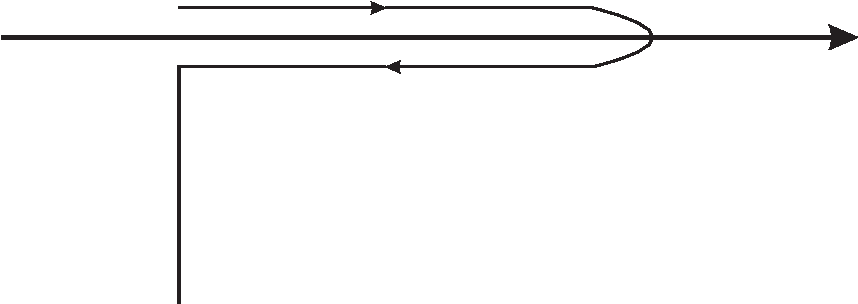
\includegraphics[width=60mm]{imagefile1a}}
\caption{The Keldysh contour before extension of the real axis to infinity
\source{}}
\end{figure}

In the next section we provide a short example manuscript, which includes images and their captions.  In \verb"sample.tex" we have added some comments explaining how to use \verb"\source{...}" to include subcaptions, and how to format equations over more than one line.  For more information on submitting and \emph{Electronics Letters} house style, see the author guide at http://www.theiet.org/resources/journals/eletters/authors.cfm.

\section{Kondo effect in new places}
With poor man's scaling \cite{1} and the success of the Bethe ansatz, the equilibrium Kondo effect has become something of a solved problem (Anderson's withering remarks concerning the Bethe ansatz notwithstanding).  However, there are two situations where it is \emph{not} properly understood.  The Kondo lattice is of particular interest in the heavy fermion compounds, and is far beyond the scope of the current work, and we refer the reader to \cite{2} and references therein.  Similarly, the case where the Kondo impurity is not in a metal but a superconductor, is not dealt with in the present work.  Of interest are non-equilibrium effects, and this is typically realized in quantum dots.

In the typical quantum dot set-up, as described in the introduction, the dot weakly connects together two electron seas, the leads.  It is understood that the phenomenon of the Coulomb blockade limits conductance through the dot unless the charge induced on the dot by the gate is
\begin{align}
  Q=\left(N+\frac{1}{2}\right)e
\end{align}
Consequently, we find sharp peaks in the conductance of the dot at these degeneracy points.  However, for $T<T_{K}$ new behaviour is observed, as in Fig. \ref{kondodotresistance}.  The original conduction peaks of figure of the classic Coulomb blockade exist when the occupancy is effectively half integer.  Hence, we expect at integer occupancy \emph{suppression} of the conductance.  This is indeed observed if $N$ is even.  However, for $T<T_{K}$ and $N$ odd, we see that the conductance is not \emph{fully} suppressed.  The difference is clear: for even occupancy, the spin of the dot will be zero, as there will be as many up as down electrons.  However, for odd filling, the $N+1$th electron will contribute a spin-half, causing the dot to behave as a Kondo-like impurity.  We will discuss what consequences the Kondo-nature of the dot has, but first we will explain exactly \emph{how} it acquires this nature.

\section{The Schrieffer-Wolff transformation}
To set up the non-equilibrium Kondo problem - formally - we introduce the two-channel Anderson Hamiltonian
\begin{align}
  H_{2C}=&\sum_{\alpha k\sigma}\epsilon_{\alpha k}\hat{c}^{\dagger}_{\alpha k\sigma}\hat{c}_{\alpha
  k\sigma}+U\hat{d}^{\dagger}_{\uparrow}\hat{d}_{\uparrow}\hat{d}^{\dagger}_{\downarrow}\hat{d}_{\downarrow}\nonumber\\
  &+\sum_{\sigma}\epsilon_{d}\hat{d}^{\dagger}_{\sigma}\hat{d}_{\sigma}+\sum_{\alpha
  k\sigma}[t_{\alpha}\hat{c}^{\dagger}_{\alpha k\sigma}\hat{d}_{\sigma}+h.c.]
\end{align}
The subscript $\alpha$ is the channel label, for the dot case left and right.  The physical idea is that the dot is already at half-integer occupancy.  The Hubbard $U$ is recognized as the charging energy (the energy required to add another electron) which we assume to be much larger than the mean level spacing in the dot, so that we may consider only one level, $\epsilon_{d}$.  The hybridization, $t_{\alpha}$ is the tunneling energy through the potential barriers connecting the dot to the leads, and is assumed to be point like.  It is clear that the dot behaves exactly as the original Anderson impurity model, with the addition of lead indices, and this Hamiltonian has been studied \emph{perturbatively}.  However, the Schrieffer-Wolff transformation can be performed exactly as before:
\begin{align}
  H_{2K}=\sum_{\alpha k\sigma}\epsilon_{\alpha k}\hat{c}^{\dagger}_{\alpha k\sigma}\hat{c}_{\alpha
  k\sigma}+\sum_{\alpha\beta\sigma\tau}\underbrace{\frac{t^{*}_{\alpha}t_{\beta}}{U}}_{J_{\alpha\beta}}\hat{c}^{\dagger}_{\alpha\sigma}(r=0)\sigma^{a}_{\sigma\tau}\hat{c}_{\beta\tau}(r=0)S^{a}
\end{align}
In the following we will assume that the coupling to the left and right leads is identical, $J_{\alpha\beta}$,  we may perform the sum over leads, giving
\begin{align}\label{2lead}
  H_{2K}=\sum_{\alpha k\sigma}\epsilon_{\alpha k}\hat{c}^{\dagger}_{\alpha k\sigma}\hat{c}_{\alpha
  k\sigma}+J\{[\hat{c}_{L\sigma}^{\dagger}(r=0)+\hat{c}_{R\sigma}^{\dagger}(r=0)]\nonumber\\
  \times\sigma^{a}_{\sigma\tau}[\hat{c}_{L\tau}(r=0)+\hat{c}_{R\tau}(r=0)]\}S^{a}
\end{align}

\begin{figure}
\centering{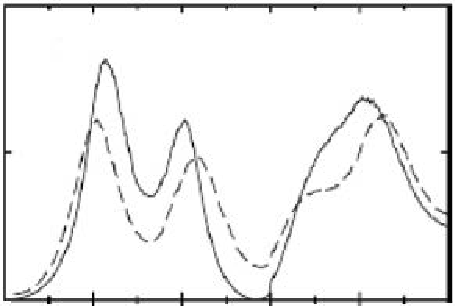
\includegraphics[width=60mm]{imagefile2a}}
\caption{Quantum dot resistance for $T\ll T_{K}$ and $T\gg T_{K}$
\source{For  high temperatures (dashed line) the Coulomb blockade remains}
\source{For lower temperatures (solid line) the Coulomb blockade is overcome}}\label{kondodotresistance}
\end{figure}


\section{Some Simple Results for Two Leads}
If we assume that the kinetic term takes the same form for the left lead as the right lead (in equilibrium), a simple (Bogoliubov) rotation of basis will transform $H_{2K}$ into the standard one channel Kondo model:
\begin{align}\label{kondolies}
  \hH_{2K}^{1}=\sum_{k}\varepsilon_{k}\hat{c}_{\alpha k\sigma}\D\hat{c}_{\alpha k\sigma}+
  J\sum_{\alpha}\hat{s}(0)\cdot\hat{S}
\end{align}
such that the new Hamiltonian is diagonal in the lead index, and so $\alpha$ behaves as an additional degeneracy.  This procedure is justified if we wish to \emph{perturbatively} analyze the conductance of the dot.  For bias voltages, $V$ much lower than the Kondo temperature, this seems reasonable, as the only true energy scale for the Kondo model is $T_{K}$.

Given that $\hH_{2K}^{1}$ is diagonal in lead index, the same techniques as are used for the equilibrium case apply.  Indeed, performing the poor man's scaling procedure and using Fermi's golden rule, it is straightforward to recover the result, for $T\gg T_{K}$:
\begin{align}
  &G_{1}\sim G_{0}\nu_{0}J\nonumber\\
  &G_{0}\sim{\ln^{2}(T/T_{k})}
\end{align}
A full and more careful treatment, recovers the numerical factors:
\begin{align}
  G_{1}&=\frac{2e^{2}}{h}\frac{4\Gamma_{L}\Gamma_{R}}{(\Gamma_{L}+\Gamma_{R})^{2}}\frac{3\pi^{2}/16}{\ln^{2}(T/T_{k})}\nonumber\\
  &\equiv G_{0}\frac{3\pi^{2}/16}{\ln^{2}(T/T_{k})}
\end{align}
We emphasize that this is valid \emph{only} for $T\gg T_{K}\gg V$.

At temperatures below $T_{K}$, the coupling diverges, so that the dominant term in equation (\ref{kondolies}) is
\begin{align}
  \hH_{coup}=J\sum_{\alpha}\hat{s}(0)\cdot\hat{S}
\end{align}
As was discussed for the one channel problem, the ground state is a singlet, with zero spin, and we expect the scattering in the dot to be suppressed, and so to leading order, the the conductance reduces to $G_{2}=G_{0}$.  Perturbative corrections have been found, \cite{3}, which yield
\begin{align}
  G_{2}=G_{0}\left[1-\left(\frac{\pi T}{T_{K}}\right)^{2}\right]
\end{align}
Thus, we can define two regions for the conductance, both for $V\ll T_{K}$:
\begin{align}
  \begin{array}{cc}
    G_{1}=G_{0}\frac{3\pi^{2}/16}{\ln^{2}(T/T_{k})}, & \;\;\;\;T\gg T_{K} \\
    G_{2}=G_{0}, & \;\;\;\;T\ll T_{K}
  \end{array}
\end{align}
So, we see that as we lower the temperature below $T_{K}$, for an odd-integer Coulomb blockade valley, the conductance is no longer exponentially suppressed.

As we have stressed, these results are valid \emph{only} for $V\ll T_{K}$.  The next step is to introduce an arbitrary voltage via the kinetic term in equation (\ref{kondolies}):
\begin{align}
  \hH_{2K}^{1}=\sum_{k\sigma}(\varepsilon_{k}-eV)\hat{c}_{L k\sigma}\D\hat{c}_{L k\sigma}+
  \sum_{k\sigma}\varepsilon_{k}\hat{c}_{R k\sigma}\D\hat{c}_{R k\sigma}+
  J\sum_{\alpha}\hat{s}(0)\cdot\hat{S}
\end{align}
If we assume that $V\gg T$, we can again divide into two regions:
\begin{align}
  \tilde{G}=\left\{\begin{array}{cc}
     \tilde{G}_{1}, & \;\;\;\;\;\;\;V\gg T_{K} \\
     \tilde{G}_{2}, & \;\;\;\;\;\;\;V\ll T_{K}
   \end{array}\right.
\end{align}
Here, the previous work is based on the idea that $eV$ now plays the same role as temperature.  That is, in the R.G. flow, we cut at $eV$, and the perturbation analysis of \cite{3} is now for low voltage, so we find
\begin{align}
     &\tilde{G}_{1}=G_{0}\frac{3\pi^{2}/16}{\ln^{2}(eV/T_{k})}\nonumber\\
     &\tilde{G}_{2}=G_{0}\left[1-\left(\frac{\pi eV}{T_{K}}\right)^{2}\right]
\end{align}
However, we argue that the approximations used are not entirely reasonable.  From the work of N. d'Ambrumenil and B. Muzykantskii, on the non-equilibrium x-ray problem (to which the Kondo problem can be related), it is \emph{not} sufficient to decouple the leads, rotate basis and then simply reintroduce the voltage.  It is clear (in the very least as a precaution), that a full treatment of the \emph{true} two lead Kondo Hamiltonian of equation (\ref{2lead}) is required.  With this in mind, in the next chapter, we will be following the calculation of Anderson, Yuval and Hamann, in which they map the Kondo Hamiltonian onto a two dimensional Coulomb gas.

%\vfill\pagebreak

\section{Conclusion}
We have derived some results for the two lead Kondo problem in various limits.  We have shown the suppression of the Coulomb blockade, and observed that this suppression can be viewed as a kind of delocalisation caused by the Kondo singlet across the dot.  The above treatment required us to neglect the bias potential and then to rotate our two lead problem to a diagonal basis.  However, it is not clear that this is a controlled or reasonable approach.  In fact, the presence of voltage in the non-diagonal Green's function of related x-ray problems implies that the voltage cannot be treated perturbatively, and that a generalisation of non-eequilibrium Riemann-Hilbert techniques may be necessary.
\vskip3pt
\ack{This work has been supported by The IET}

\vskip5pt

\noindent J. Smith and A. N. Other (\textit{The IET, Stevenage, UK})
\vskip3pt

\noindent E-mail: jsmith@theiet.org

\begin{thebibliography}{}

\bibitem{1}
Anderson, P.: `A poor man's derivation of scaling laws for the Kondo problem', \textit{J. Phys. C.}, 1960, \textbf{3}, p. 2436

\bibitem{2}
Coleman, P.: `1/N expansion for the Kondo lattice', \textit{Phys. Rev. B}, 1983, \textbf{28}, pp. 5255-5262

\bibitem{3}
Ludwig, I. and Ludwig A. W. W.: `Kondo effect induced by a magnetic field', \textit{Phys. Rev. B}, 2001, \textbf{64}, p. 045328

\end{thebibliography}

\end{document}

%\begin{table}[b]
%\processtable{Coefficients and remainders for distribution KK ($k = 0.05$,
%$v = 3$, $c_{1} = 1.5$, $c_{2} = 4.5$)}
%{\begin{tabular}{|l|l|l|}\hline
%$n$ & $a_{n}^{2}$ & $r_{k}(1)$\\\hline
%0 & 3.602576748428 & 1.493719547999\\\hline
%1 & 1.384791111989 & 0.108928436101\\\hline
%2 & 0.108600438794 & 0.000327997399\\\hline
%3 & 0.000275794597 & 0.000052202814\\\hline
%4 & 0.000027616892 & 0.000024585922\\\hline
%5 & 0.000018178621 & 0.000006407300\\\hline
%\end{tabular}}{}
%\end{table}
%
%So, the basic preamble and main body will be:
%\verb"\documentclass[twocolumn]{el-author}"\\
%\verb"\usepackage[...]{packages}"\\
%\verb"\date{12 December 2012}"\\
%\verb"\title{...}"\\
%\verb"\author{...}"\\
%\verb"\abstract{...}"\\
%\verb"\maketitle{...}"\\
%\verb"\begin{document}"\\
%\verb"..."\\
%\verb"\section{...}"\\
%\verb"..."\\
%\verb"\section{..}"\\
%\verb"..."\\
%\verb"\end{document}"
